\documentclass[14pt,aspectratio=169]{beamer}

\usepackage{pgfpages}
\usepackage{fancyvrb}

\usepackage{tikz}
\usepackage{pgfplots}

\usepackage{minted}
\usemintedstyle{tango}

\usepackage{graphicx}

\usetheme{auriga}
\usecolortheme{auriga}

\setbeamercolor{background canvas}{bg=lightgray}

% define some colors for a consistent theme across slides

\definecolor{red}{RGB}{181, 23, 0}
\definecolor{blue}{RGB}{0, 118, 186}
\definecolor{gray}{RGB}{146, 146, 146}

\title{Web Development: \\ Using Color and Web Media}

\author{{\bf Gregory M. Kapfhammer}}

\institute[shortinst]{{\bf Department of Computer Science, Allegheny College}}

\begin{document}

{
  \setbeamercolor{page number in head/foot}{fg=background canvas.bg}
  \begin{frame}
    \titlepage
  \end{frame}
}

% Slide
%
\begin{frame}{Technical Question}
  %
  \hspace*{.25in}
  %
  \vspace*{.2in}
  %
  \begin{minipage}{5in}
    %
    \begin{center}
      %
      {\large How can I use HTML and CSS source code to design and implement
      multicolumn and responsive web page layouts?}
      %
    \end{center}
    %
  \end{minipage}
  %
  \vspace{2ex}
  %
  \begin{center}
    %
    \small Let's learn how to combine CSS and HTML to mobile-ready layouts for
    our web pages! We will also explore the benefits of using responsive web
    design frameworks like Bootstrap. Make sure to review all previous
    content!\\
    %
  \end{center}
  %
\end{frame}

% Slide
%
\begin{frame}{The Normal Flow of Web Page Layout}
  %
  \begin{itemize}
    %
    \item How does the web browser normally layout the block-level and inline
      elements from left to right and top to bottom?
      %
      \vspace*{-.15in}
      %
    \item The fundamental components of a web page:
      %
      \begin{itemize}
        %
        \item {\bf Block-level elements}: content contained on their own line
          %
        \item {\bf Inline elements}: content displayed within an existing line
          %
          \begin{itemize}
            %
            \item {\bf Replaced}: content defined by an external resource
              %
            \item {\bf Non-replaced}: content defined by an in-document
              resources
              %
          \end{itemize}
          %
      \end{itemize}
      %
      \vspace*{-.2in}
      %
    \item How can you tell if a component is block-level or not?
      %
      \vspace*{-.2in}
      %
    \item How can you tell if a component is inline or not?
      %
      \vspace*{-.2in}
      %
    \item When is an element replaced versus non-replaced?
      %
  \end{itemize}
  %
\end{frame}

% Slide
%
\begin{frame}[fragile]
  \frametitle{Identifying Block-Level and Inline Content}
  \normalsize
  \begin{minipage}{6in}
    \vspace*{.1in}
    \begin{minted}[mathescape, numbersep=5pt, fontsize=\large]{html}
<h3>Photograph Reviews</h3>
<blockquote>
  <p><b>By Ricardo on
     <time>February 8, 2018</time></b>
  </p>
  <p>That is a great photograph!</p>
  <p>I would describe this as
     <i class="em em---1"></i></p>
</blockquote>
    \end{minted}
  \end{minipage}
%
\end{frame}

% Slide
%
\begin{frame}[fragile]
  \frametitle{Finding Replaced and Non-Replaced Content}
  \normalsize
  \begin{minipage}{6in}
    \vspace*{.2in}
    \begin{minted}[mathescape, numbersep=5pt, fontsize=\large]{html}

  <a title="A Delta 757 lands at LAX
      on January 29th. #latergram"
  href="https://flickr.com/photos/
        pt737swa/28371915769">
      <img src="img/plane.jpg"/>
  </a>

    \end{minted}
  \end{minipage}
  %
  \vspace*{.1in}
  %
  \begin{center}
    Which content would we categorize as being replaced?
  \end{center}
\end{frame}

% Slide
%
\begin{frame}{Layout of Block-Level and Inline Content}
  %
  \begin{itemize}
    %
    \item Block-level elements stack {\bf top to bottom}
      %
      \vspace*{-.2in}
      %
    \item Inline elements layout {\bf left to right}
      %
      \vspace*{-.2in}
      %
    \item Block-level {\bf has} its own container
      %
      \vspace*{-.2in}
      %
    \item Inline content {\bf exists in} a container
      %
      \vspace*{-.2in}
      %
    \item Content layout in HTML and CSS:
      %
      \begin{itemize}
        %
        \item Browsers adhere to default rules for all HTML elements
          %
        \item Web developers can modify these defaults through CSS
          %
        \item Incorrect redefinitions can lead to layout faults
          %
        \item Layout faults can manifest in layout failures!
          %
      \end{itemize}
      %
  \end{itemize}
  %
\end{frame}

% Slide
%
\begin{frame}[fragile]
  \frametitle{Redefining an Element's Layout with CSS}
  \normalsize
  \hspace*{.15in}
  \begin{minipage}{6in}
    \vspace*{.2in}
    \begin{minted}[mathescape, numbersep=5pt, fontsize=\small]{html}
<p>I am a paragraph. A short one.</p>
<ul>
  <li>Item One</li>
  <li>Item Two</li>
  <li>Item Three</li>
</ul>
<p>I am another paragraph.
Some of the <span class="block">words</span>
have been wrapped in a <span>span element</span>.</p>
    \end{minted}
  \end{minipage}
  \vspace*{.05in}
  \begin{center}
    %
    \noindent What is the meaning of {\tt class="block"}? \\
    %
    \noindent  \url{https://developer.mozilla.org/en-US/docs/Learn/CSS/Building_blocks/The_box_model}
    %
  \end{center}
  %
\end{frame}

% Slide
%
\begin{frame}[fragile]
  \frametitle{Controlling the Display of Content with CSS}
  \normalsize
  \hspace*{.25in}
  \begin{minipage}{6in}
    \vspace*{.2in}
    \begin{minted}[mathescape, numbersep=5pt, fontsize=\large]{css}
.block {
  display: block;
}
    \end{minted}
  \end{minipage}
  \vspace*{.05in}
  \begin{center}
    %
    \noindent What is the HTML tag that this selector styles? \\
    %
    \noindent Can you find the key value pairs in this CSS code? \\
    %
    \noindent How does {\tt display: block;} change the normal flow? \\
    %
    \noindent Remember, HTML elements are either {\bf block} or {\bf inline}! \\
    %
  \end{center}
  %
\end{frame}

% Slide
%
\begin{frame}{Positioning of HTML Elements}
  %
  \begin{itemize}
    %
    \item It is possible to move an element away from its position in the normal
      flow. You can even move an element off of the web page itself! Why would
      a web developer do that?
      %
      \vspace*{-.15in}
      %
    \item The values for the position of an HTML element:
      %
      \begin{itemize}
        %
        \item {\bf Absolute}: removed from flow and placed relative to its
          container
          %
        \item {\bf Fixed}: forced to stay in a specific position regardless of
          scrolling
          %
        \item {\bf Relative}: removed from flow and placed relative to first
          location
          %
        \item {\bf Static}: default behavior positions an element with
          normal flow
          %
      \end{itemize}
      %
      \vspace*{-.2in}
      %
    \item What entity performs this placement? The web browser!
      %
      \vspace*{-.2in}
      %
    \item Use CSS to apply a position to an HTML element
      %
  \end{itemize}
  %
\end{frame}

% Slide
%
\begin{frame}[fragile]
  \frametitle{Using CSS Media Queries with Fixed Positioning}
  \normalsize
  \begin{minipage}{6in}
    \vspace*{.1in}
    \begin{minted}[mathescape, numbersep=5pt, fontsize=\large]{css}
  @media (min-width: 768px) {
    .back-to-top {
      position: fixed;
      bottom: 1.25rem;
      right: 0rem;
      padding: 1.25rem;
    }
  }
    \end{minted}
  \end{minipage}
%
\end{frame}

% Slide
%
\begin{frame}{Using Firefox to Inspect Fixed Positioning}
  %
  \begin{figure}
    \centering
    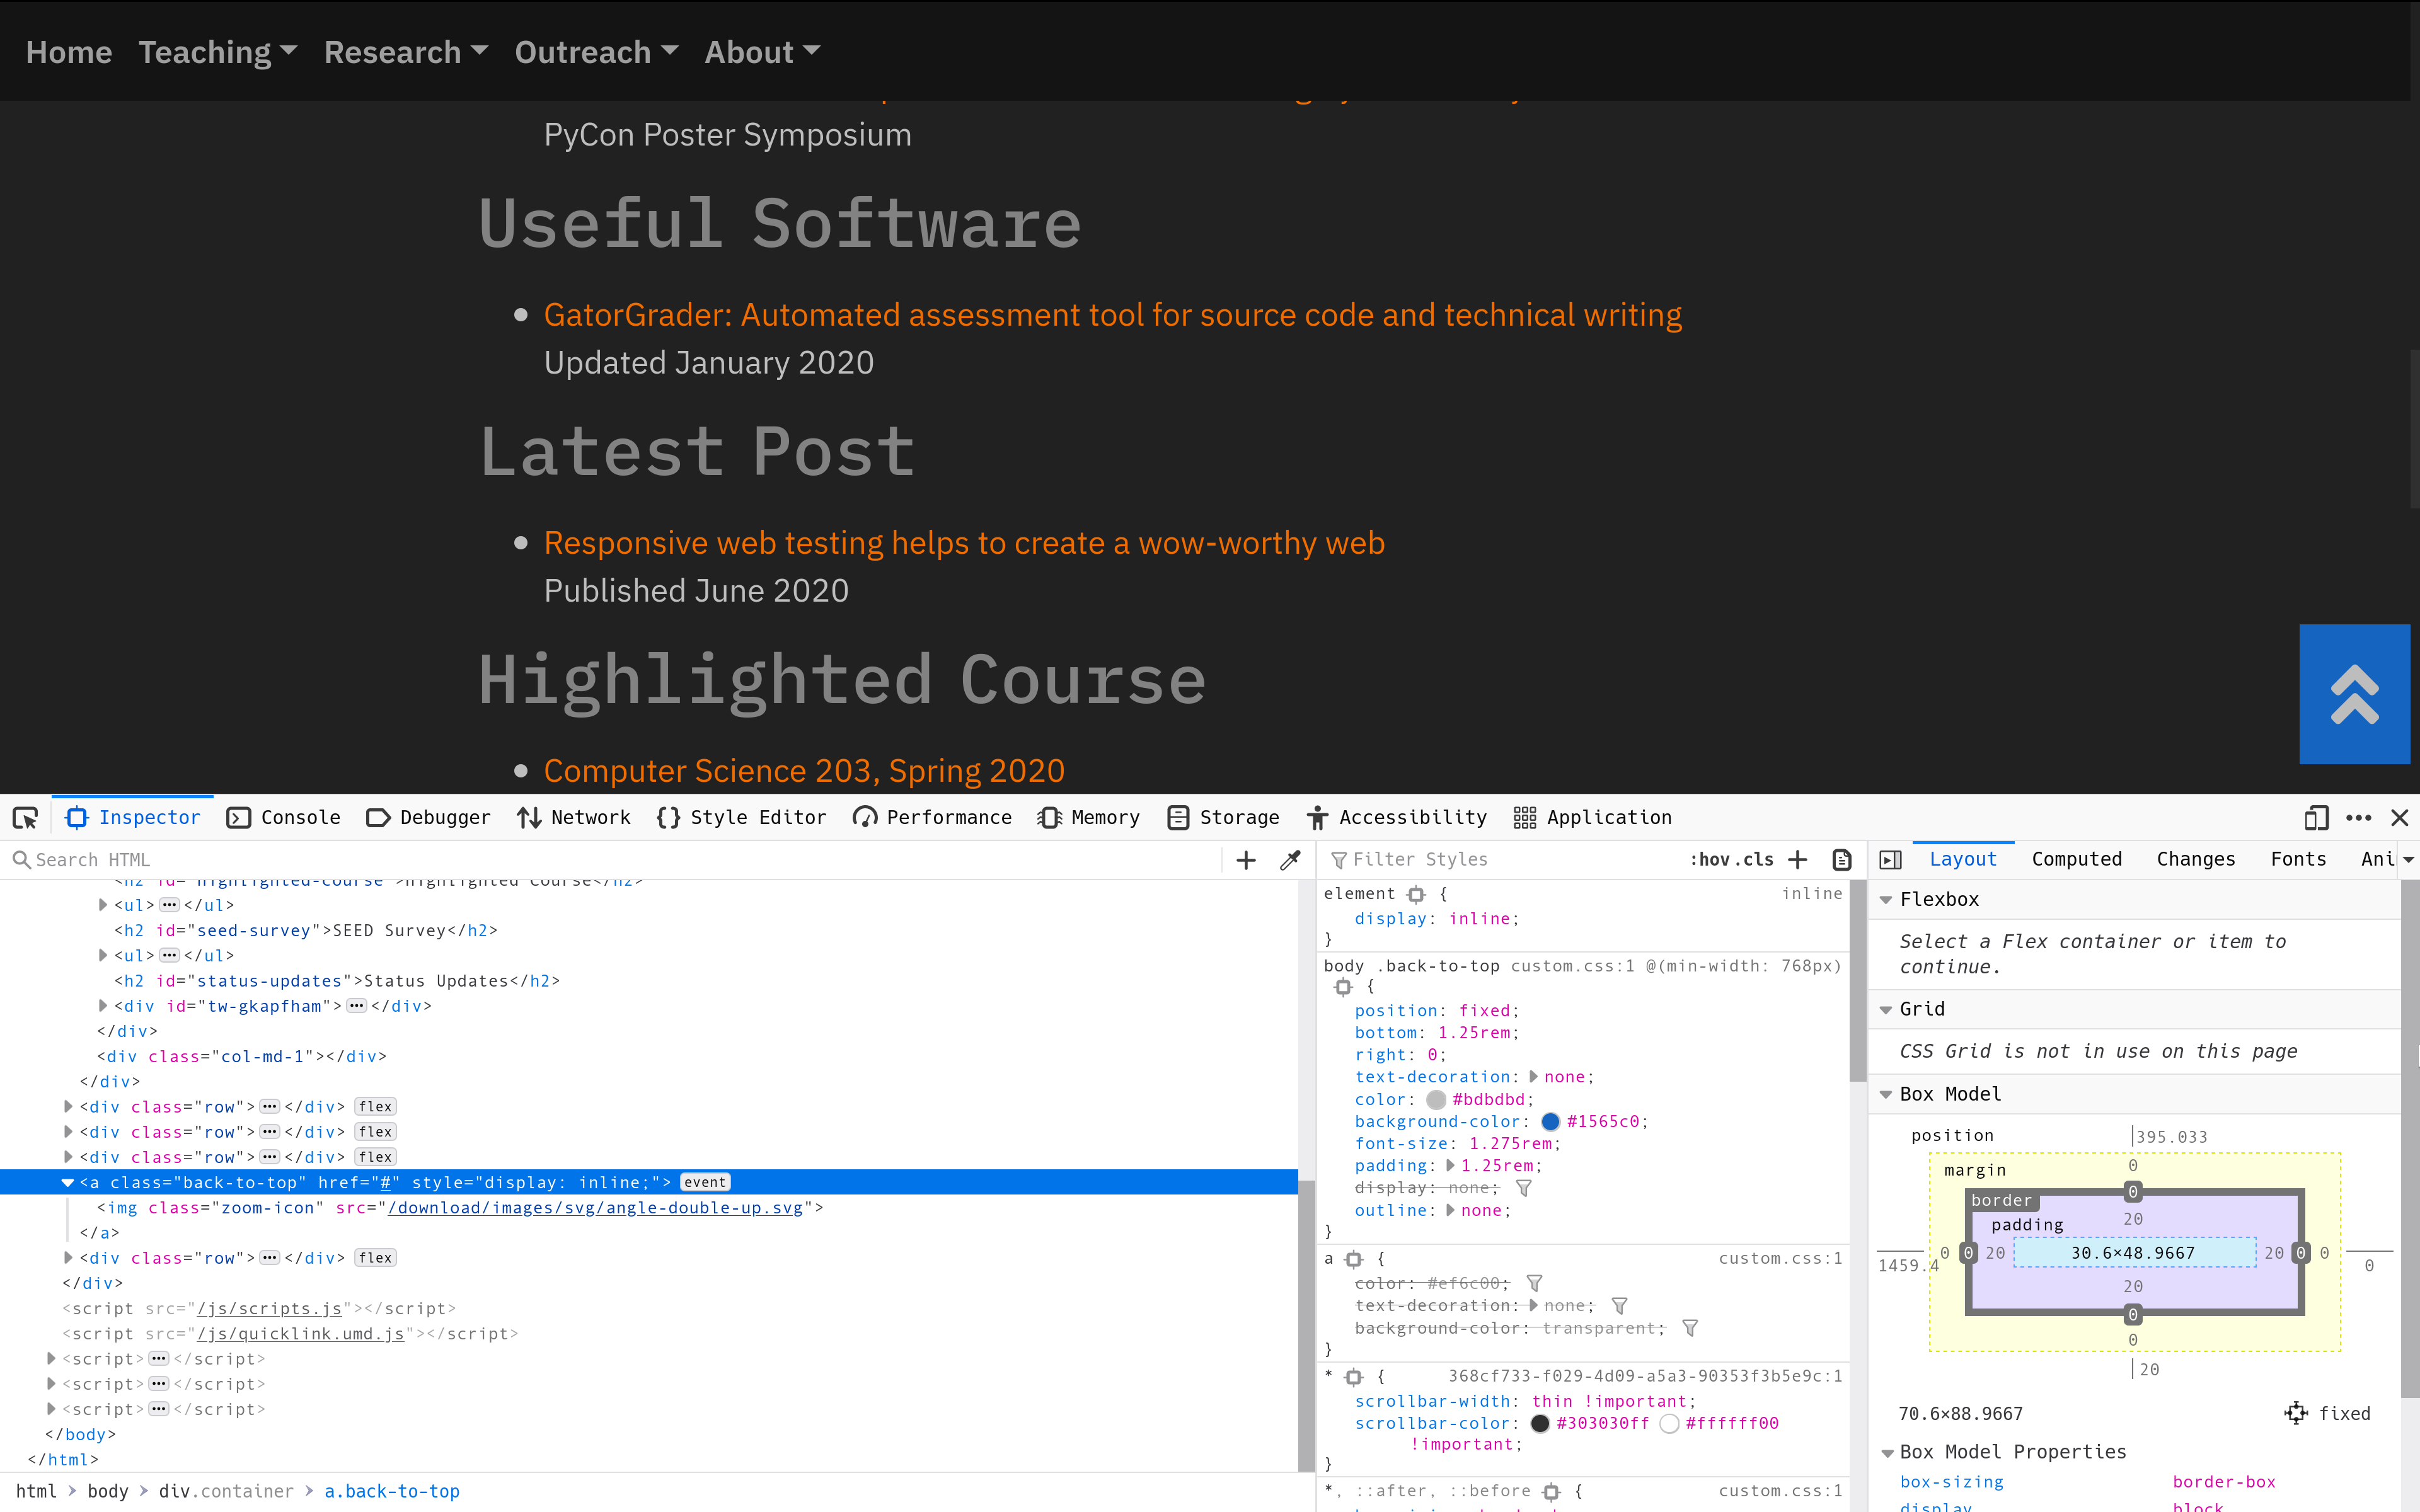
\includegraphics[scale=.08]{images/fixed-firefox.png}
    \caption{The figure's caption}
  \end{figure}
  %
\end{frame}

% Slide
%
\begin{frame}[fragile]
  \frametitle{Using Float Specifications in CSS}
  \normalsize
  \begin{minipage}{6in}
    \vspace*{.1in}
    \begin{minted}[mathescape, numbersep=5pt, fontsize=\normalsize]{css}
.dropdown-menu {
  position: absolute;
  left: 0;
  display: none;
  float: left;
  min-width: 10rem;
  padding: 0.5rem 0;
  margin: 0.125rem 0 0;
  font-size: 1.275rem;
  text-align: left;
  background-color: #141414;
}
    \end{minted}
  \end{minipage}
%
\end{frame}

% Slide
%
\begin{frame}{HTML Element Displacement through Floating}
  %
  \begin{itemize}
    %
    \item It is possible to displace an HTML out of normal flow by floating it
      to the {\tt left} or the {\tt right}. Reflows content!
      %
      \vspace*{-.15in}
      %
    \item What happens if you want to float multiple HTML elements? Or, overlay
      or hide HTML elements?
      %
      \vspace*{-.15in}
      %
    \item What if you want to design a multiple column layout?
      %
      \vspace*{-.15in}
      %
    \item Creating complex layouts is difficult when you can only use floating.
      You often have to resort to ``hacks'' to achieve the correct layout. But,
      will it work correctly on mobile devices? Better option for
      multiple-column layouts?
      %
  \end{itemize}
  %
\end{frame}

% Slide
%
\begin{frame}[fragile]
  \frametitle{Using Flexbox for Multiple-Column Layouts}
  \normalsize
  \begin{minipage}{6in}
    \vspace*{.2in}
    \begin{minted}[mathescape, numbersep=5pt, fontsize=\large]{html}
  <div class="flex-container">
    <div>Water</div>
    <div>Phone</div>
    <div>Wallet</div>
    <div>Passport</div>
    <div>License</div>
  </div>
    \end{minted}
  \end{minipage}
  %
  \vspace*{.05in}
  \begin{center}
    %
    \noindent Wait, what is the meaning of {\tt flex-container}? \\
    %
  \end{center}
  %
\end{frame}

% Slide
%
\begin{frame}[fragile]
  \frametitle{Specifying that an HTML Container Will Flex}
  \normalsize
  \begin{minipage}{6in}
    \vspace*{.2in}
    \begin{minted}[mathescape, numbersep=5pt, fontsize=\large]{css}
.flex-container {
  display: flex;
}
    \end{minted}
  \end{minipage}
  %
  \vspace*{.05in}
  \begin{center}
    %
    \noindent The {\tt flex-container} is specified in the CSS file! \\
    \noindent Remember, Flexbox is designed for one-dimensional layout! \\
    \noindent Want vertical and horizontal? Use CSS Grid! \\
    \noindent Want a full framework for layout and design? Use Bootstrap! \\
    \noindent Reference: \url{https://css-tricks.com/snippets/css/a-guide-to-flexbox/} \\
    %
  \end{center}
  %
\end{frame}

% Slide
%
\begin{frame}{Exploring Responsive Web Design}
  %
  \begin{itemize}
    %
    \item Web page layouts can either be {\bf fixed}, {\bf liquid}, or {\bf
      responsive}. What are the trade-offs in these approaches?
      %
      \vspace*{-.15in}
      %
    \item Understanding the options for web page layout:
      %
      \begin{itemize}
        %
        \item {\bf Fixed}: the web page's design assumes a specific viewport width
          %
        \item {\bf Liquid}: the layout flows to the current viewport width
          %
        \item {\bf Responsive}: the layout responds to the current viewport
          width
          %
      \end{itemize}
      %
      \vspace*{-.2in}
      %
    \item Wait, are liquid and responsive the same thing? Nope!
      %
      \vspace*{-.2in}
      %
    \item Liquid layouts often get too ``spread out'' at wide viewports
      %
      \vspace*{-.2in}
      %
    \item Responsive layouts and add, remove, and change the layout! Wow! But,
      how does that work?
      %
  \end{itemize}
  %
\end{frame}

% Slide
%
\begin{frame}[fragile]
  \frametitle{Specifying a Minimum Width in a Media Query}
  \normalsize
  \begin{minipage}{6in}
    \vspace*{.1in}
    \begin{minted}[mathescape, numbersep=5pt, fontsize=\normalsize]{css}
@media (min-width: 576px) {
  .dropdown-menu-sm-left {
    right: auto;
    left: 0;
  }
  .dropdown-menu-sm-right {
    right: 0;
    left: auto;
  }
}
    \end{minted}
  \end{minipage}
%
\end{frame}

% Slide
%
\begin{frame}[fragile]
  \frametitle{Specifying a Minimum Width in a Media Query}
  \normalsize
  \begin{minipage}{6in}
    \vspace*{.1in}
    \begin{minted}[mathescape, numbersep=5pt, fontsize=\normalsize]{css}
@media (min-width: 992px) {
  .float-lg-left {
    float: left !important;
  }
  .float-lg-right {
    float: right !important;
  }
  .float-lg-none {
    float: none !important;
  }
}
    \end{minted}
  \end{minipage}
%
\end{frame}

% Slide
%
\begin{frame}{Using CSS Grid for Responsive Web Design}
  %
  \begin{figure}
    \centering
    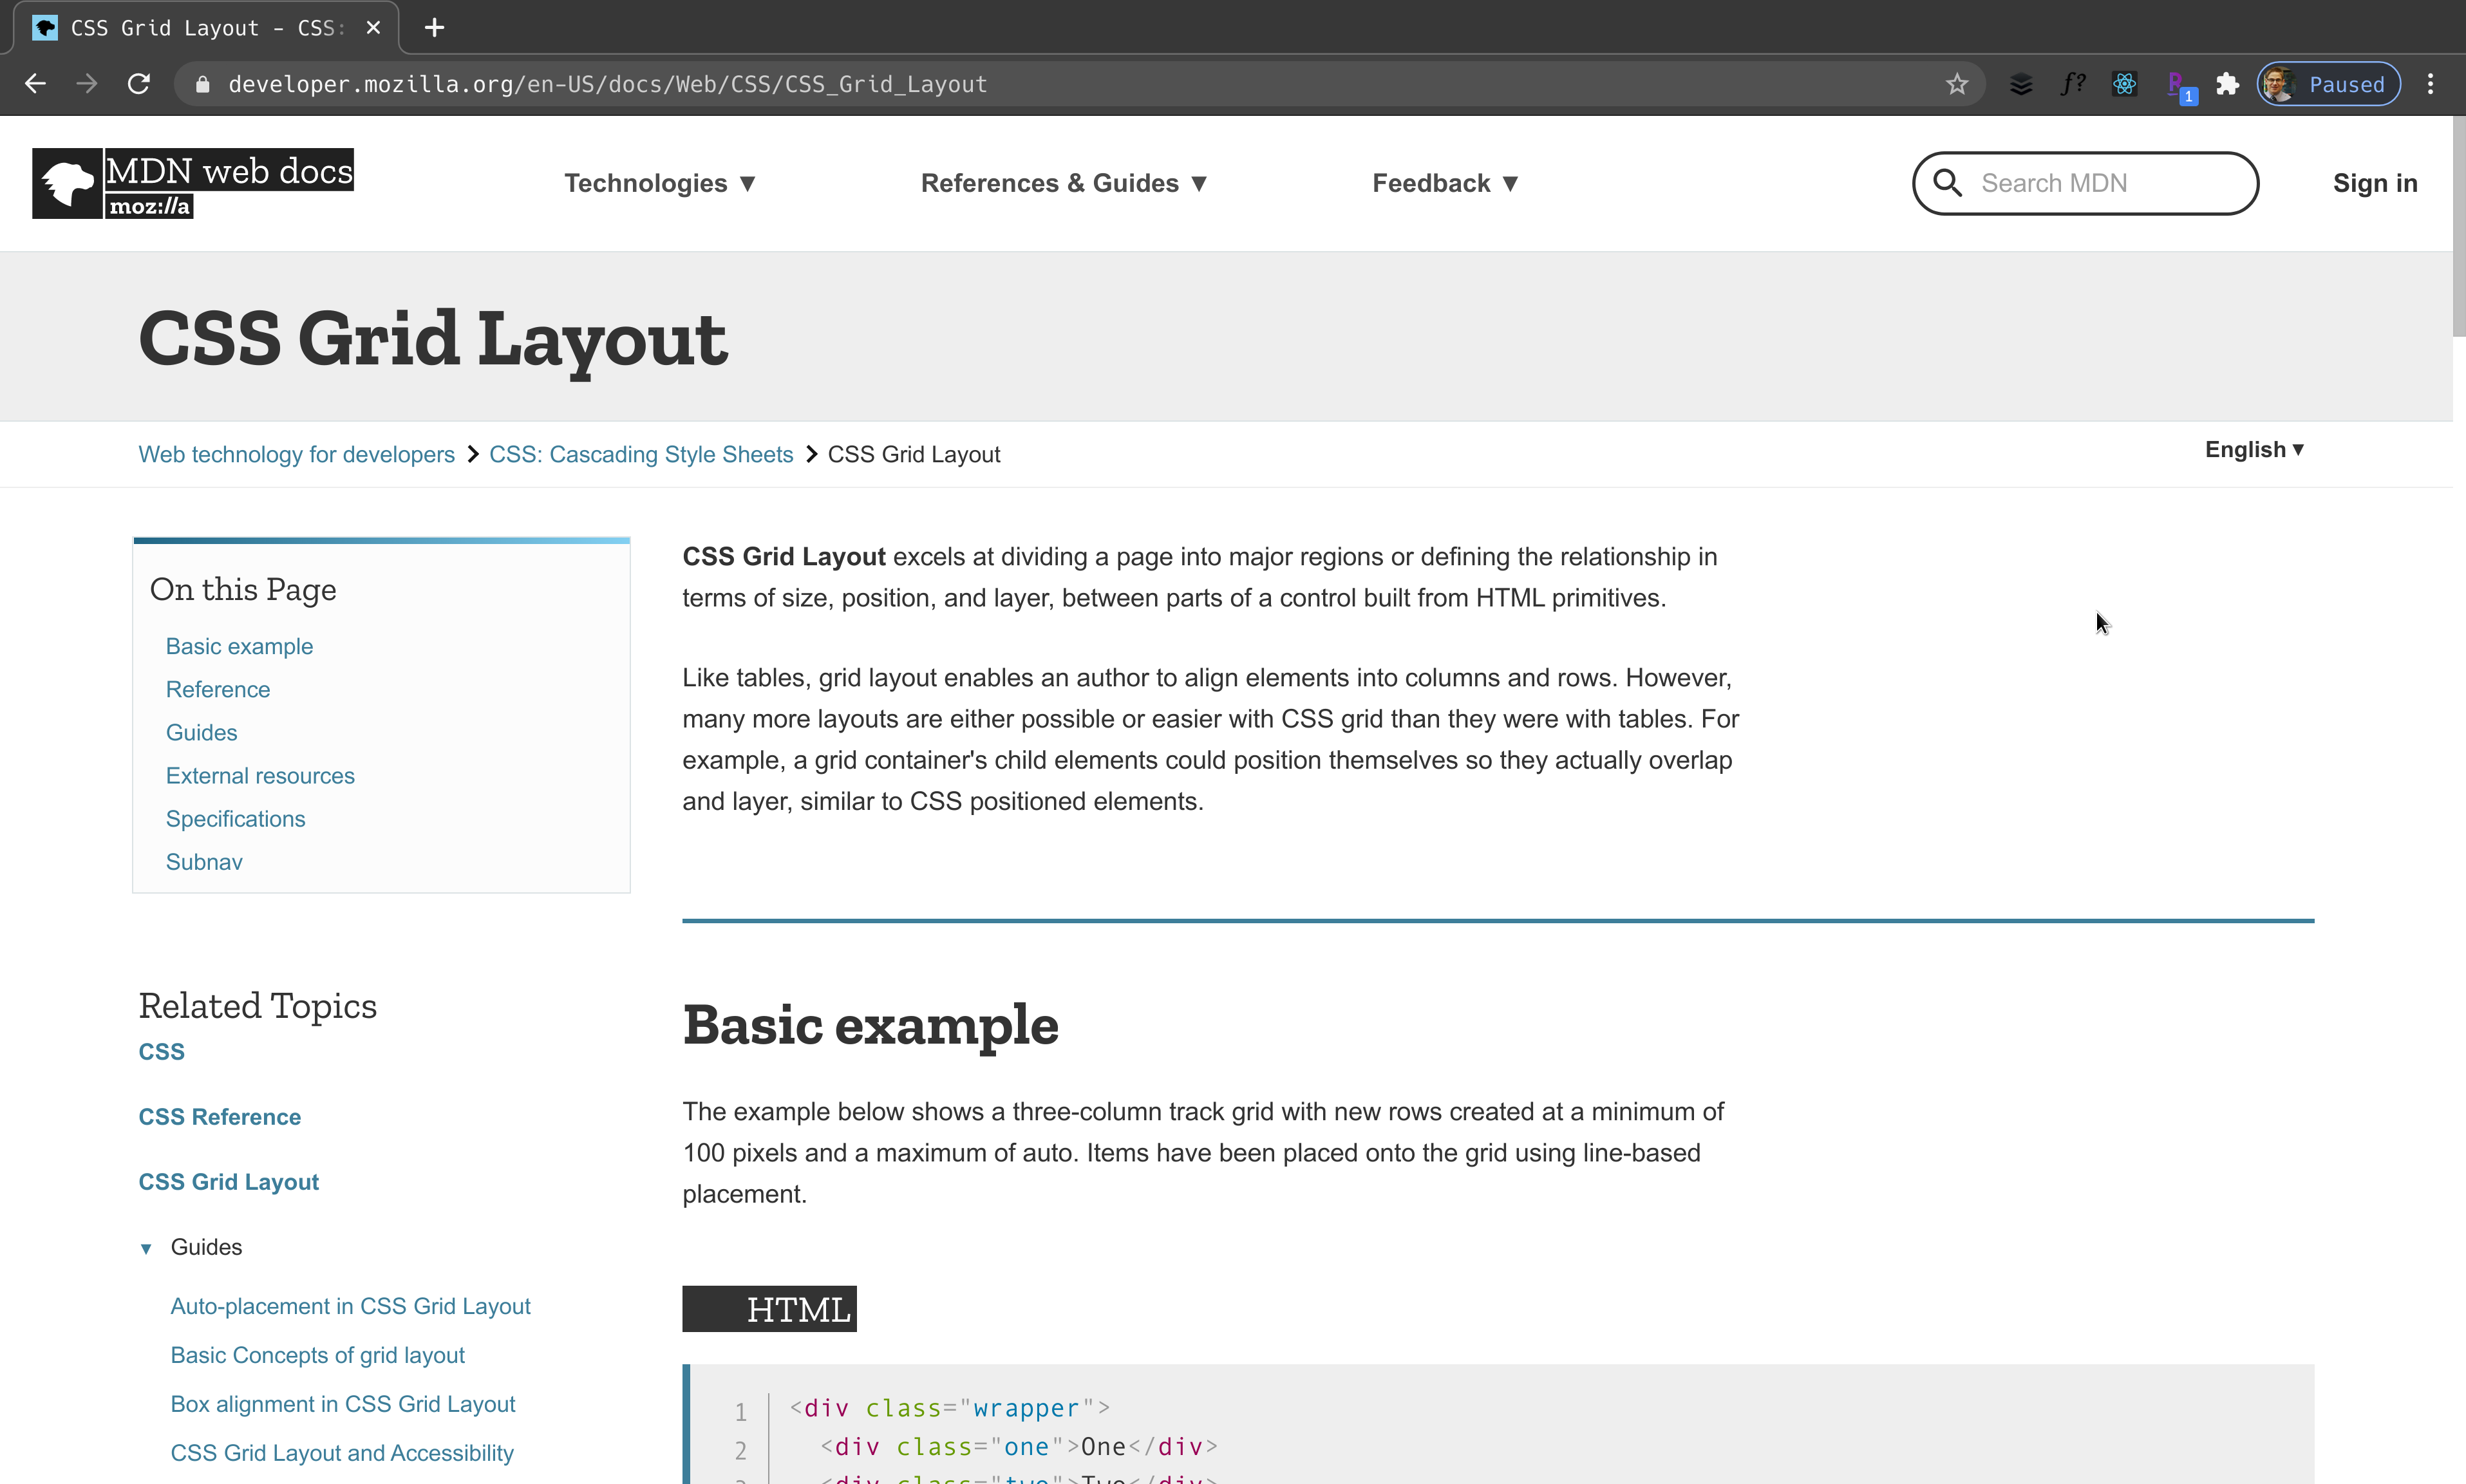
\includegraphics[scale=.085]{images/cssgrid-site.png}
    \caption{The figure's caption}
  \end{figure}
  %
\end{frame}

% Slide
%
\begin{frame}{Using Bootstrap for Responsive Web Design}
  %
  \begin{figure}
    \centering
    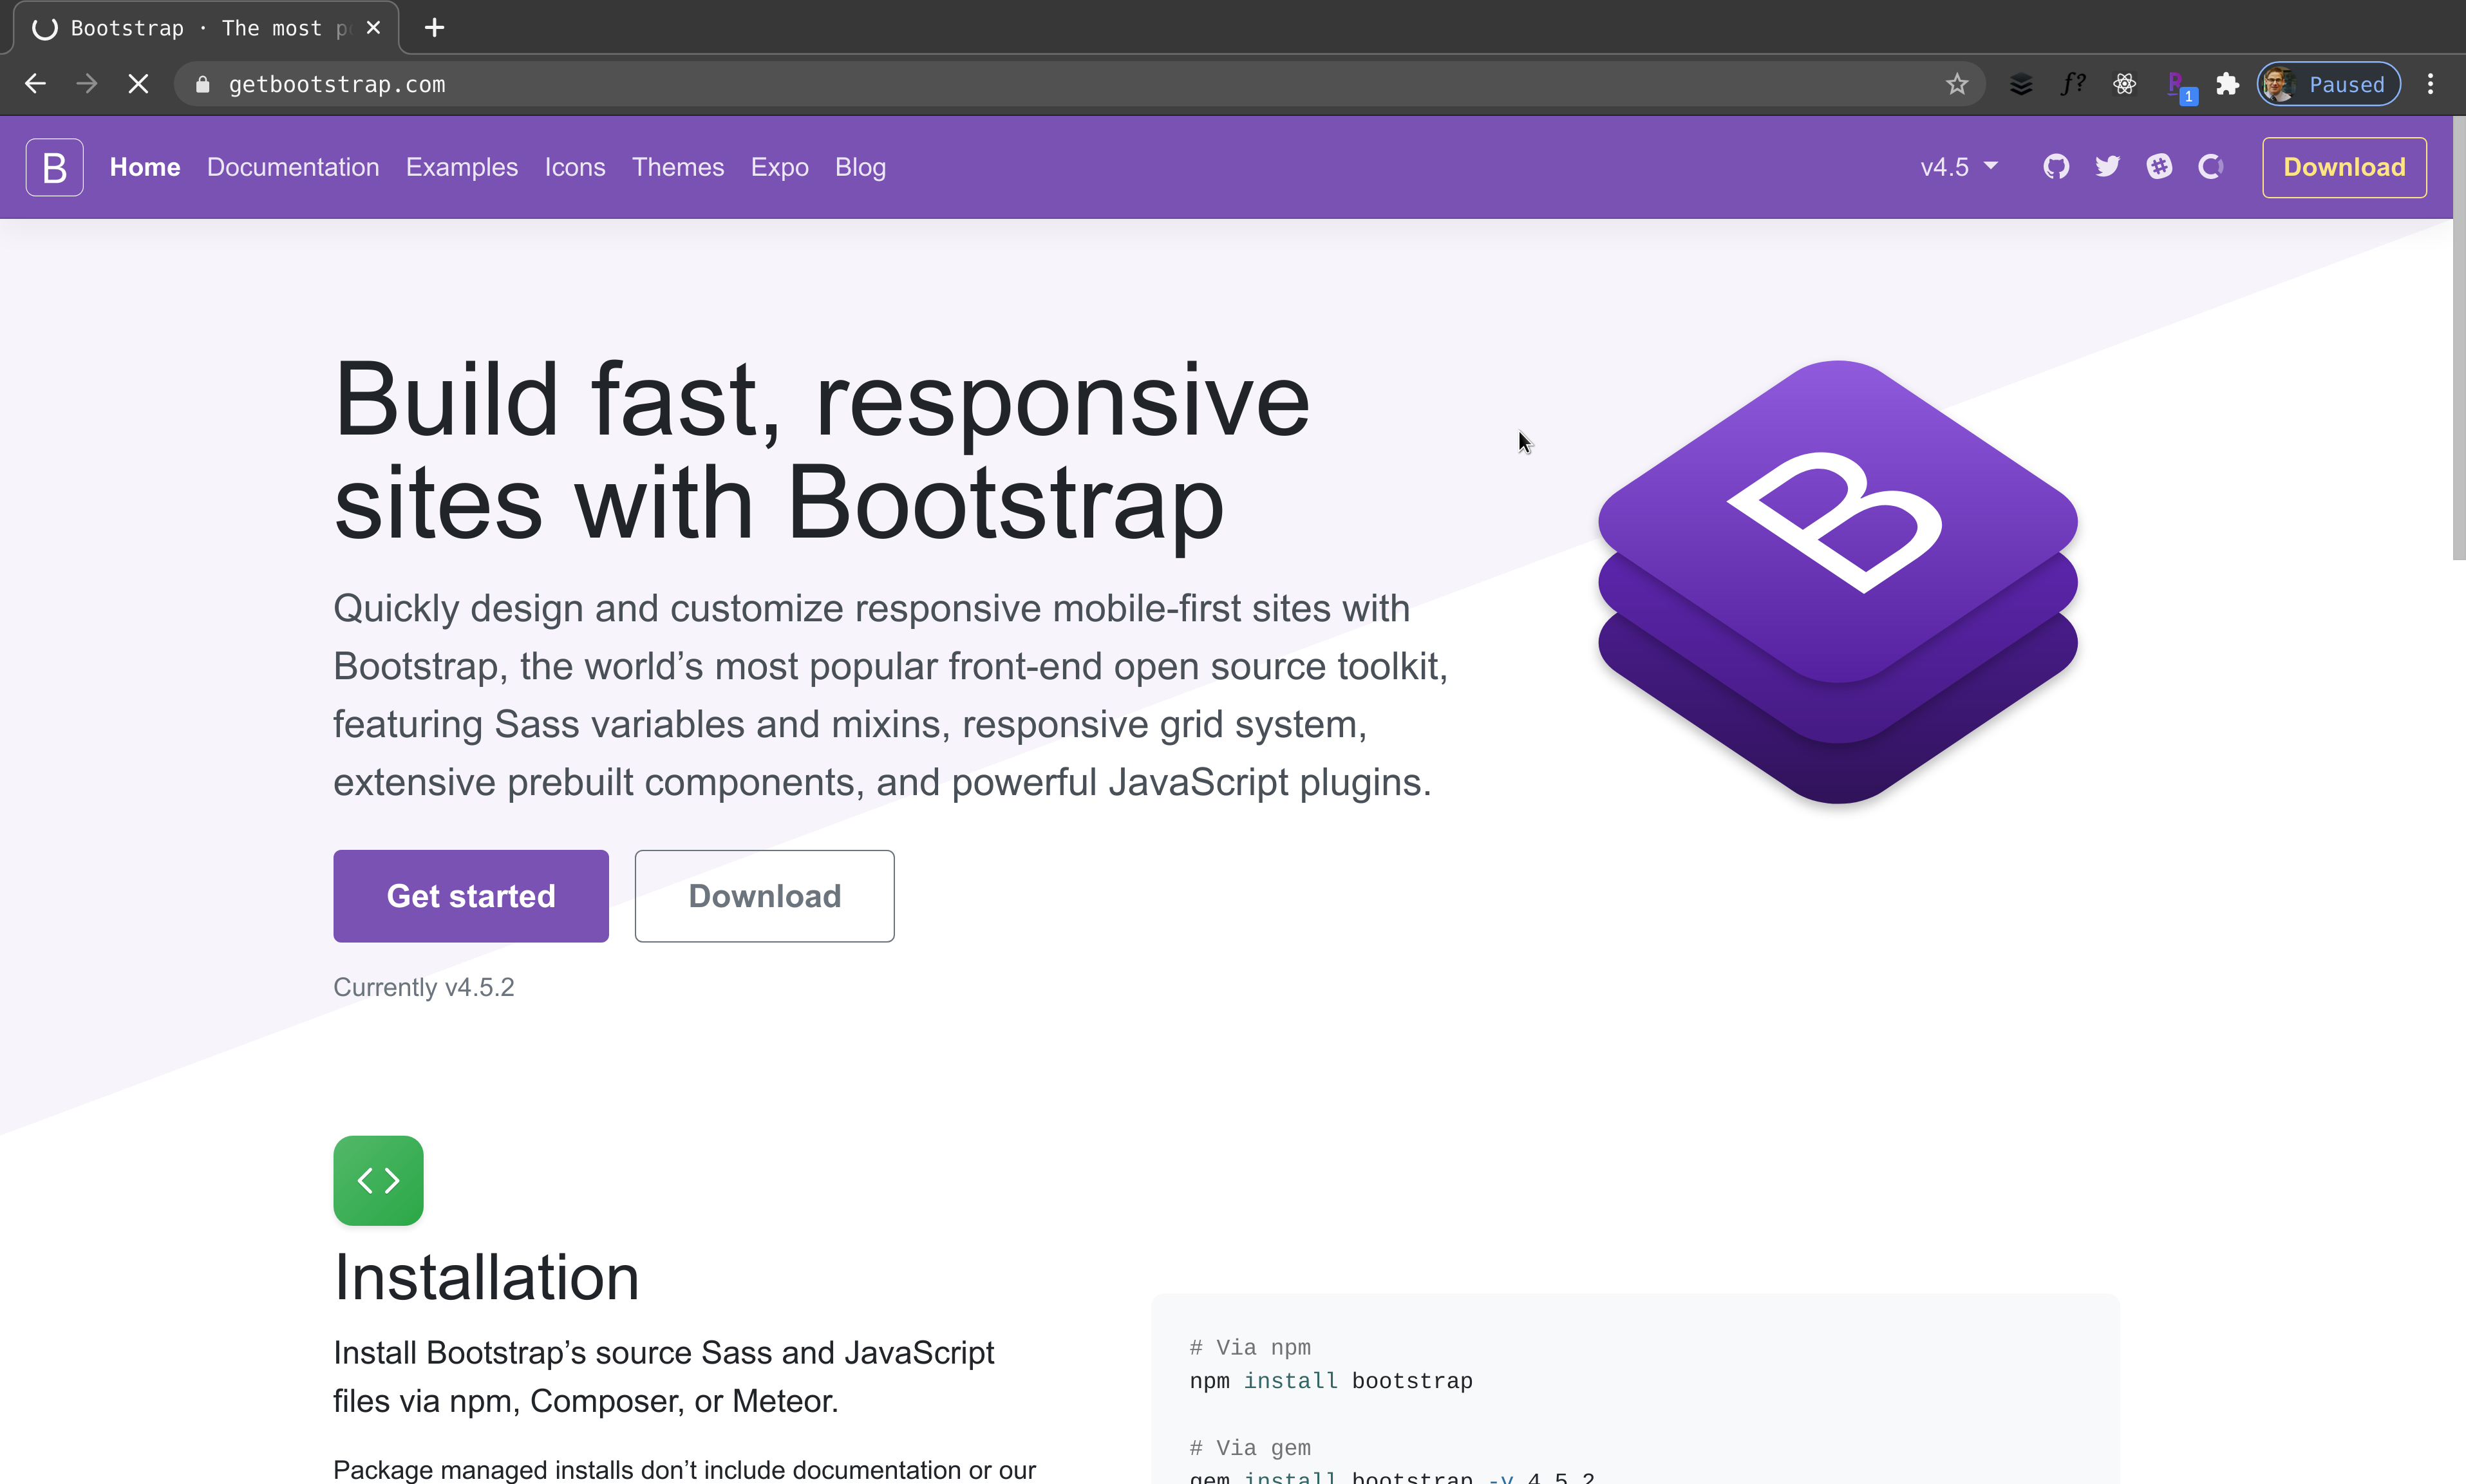
\includegraphics[scale=.085]{images/bootstrap-site.png}
    \caption{The figure's caption}
  \end{figure}
  %
\end{frame}

% Slide
%
\begin{frame}{Responsive Web Design with Bootstrap}
  %
  \begin{itemize}
    %
    \item Bootstrap defines a responsive 12-column layout
      %
      \vspace*{-.15in}
      %
    \item Media queries make a page respond to viewport width
      %
      \vspace*{-.15in}
      %
    \item Key ideas in responsive web design with Bootstrap:
      %
      \begin{itemize}
        %
        \item {\bf Viewport width}: the width of the device or browser
          %
        \item {\bf Responsive breakpoint}: the viewport widths for change
          %
        \item {\bf Media query}: conditional logic implemented in CSS
          %
      \end{itemize}
      %
      \vspace*{-.2in}
      %
    \item What are the most common viewport widths of devices?
      %
      \vspace*{-.2in}
      %
    \item How do you decide which breakpoints to implement?
      %
      \vspace*{-.2in}
      %
    \item What are the challenges of mobile-ready web design?
      %
  \end{itemize}
  %
\end{frame}

% Slide
%
\begin{frame}{Responsive Web Debugging with Firefox}
  %
  \begin{figure}
    \centering
    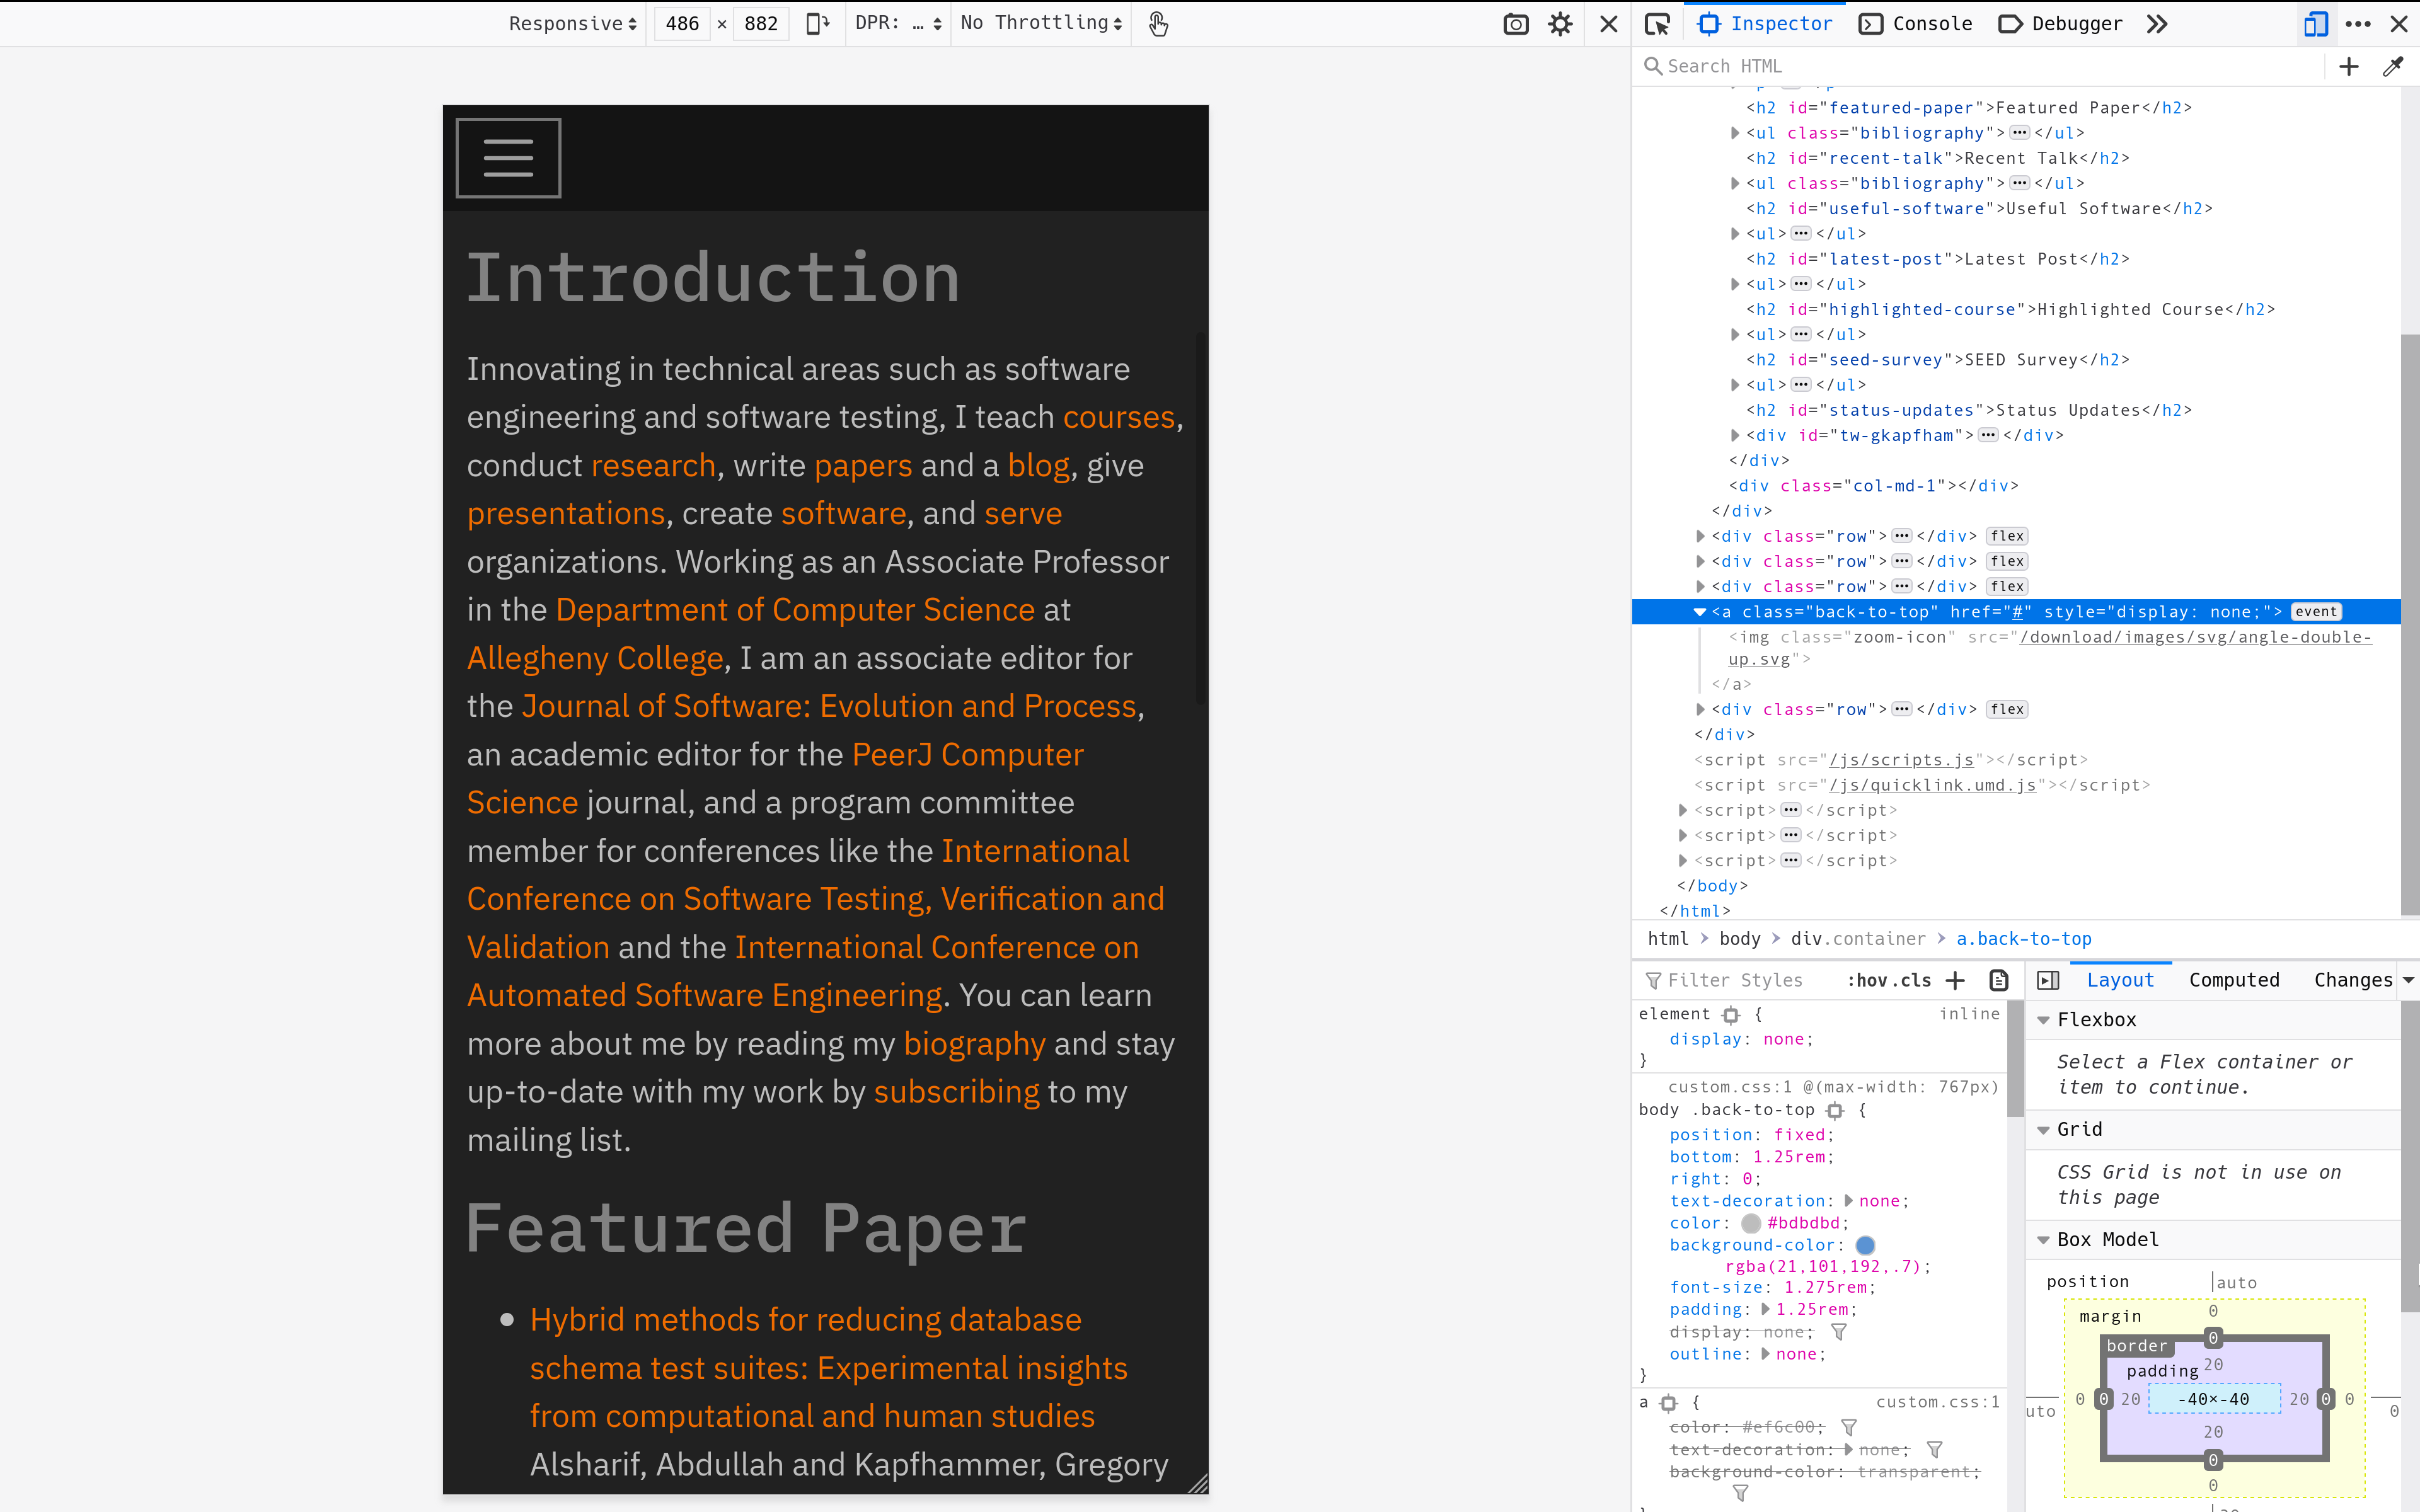
\includegraphics[scale=.085]{images/responsive-mode-firefox.png}
    \caption{The figure's caption}
  \end{figure}
  %
\end{frame}

\end{document}
